%%%%%%%%%%%%%%%%%%%%%%%%%%%%%%%%%%%%%%%%%
% Short Three-Column Newsletter
% LaTeX Template
% Version 1.0 (11/9/13)
%
% Original author:
% Frits Wenneker (http://www.howtotex.com) 
% With extensive modifications by:
% Vel (vel@latextemplates.com)
% 
% This template has been downloaded from:
% http://www.LaTeXTemplates.com
%
% License:
% CC BY-NC-SA 3.0 (http://creativecommons.org/licenses/by-nc-sa/3.0/)
%
%%%%%%%%%%%%%%%%%%%%%%%%%%%%%%%%%%%%%%%%%

%----------------------------------------------------------------------------------------
%	PACKAGES AND DOCUMENT CONFIGURATIONS
%----------------------------------------------------------------------------------------

\documentclass[10pt,a4paper,ngerman,twoside]{article} % Paper type (a4paper, usletter or legal) and font size (10, 11 or 12)

%\setlength\topmargin{-80mm} % Top margin
\setlength\topmargin{-48pt} % Top margin
\setlength\headheight{0pt} % Header height
\setlength\textwidth{7.0in} % Text width
\setlength\textheight{9.5in} % Text height
\setlength\oddsidemargin{-30pt} % Left margin
\setlength\evensidemargin{-30pt} % Left margin (even pages) - only relevant with 'twoside' article option
%\setlength\inner{4cm}
%\setlenfth\outer{2cm}
%\usepackage{geometry}
%\geometry{bindingoffset=20mm}
%\setlength\bindingoffset{2cm}

\usepackage{charter} % Charter font for main content

\frenchspacing % Reduces space after periods to make text more compact for a three-column layout
\usepackage{babel}
\usepackage[utf8]{inputenc}
\usepackage{graphicx} % Required for including images
\usepackage{amssymb} % Math packages
\usepackage{amsmath} 
\usepackage{multicol} % Required for the three-column layout of the document
\usepackage{url} % Clickable links
\usepackage{enumitem} % Reduces the amount of space within and between lists with [noitemsep,nolistsep]
\usepackage{marvosym} % Required for the use of symbols
\usepackage{wrapfig} % Allows wrapping text around figures
%\usepackage[T1]{fontenc} % Use 8-bit encoding that has 256 glyphs
\usepackage{datetime} % Required for defining a custom date style
\newdateformat{mydate}{\monthname[\THEMONTH] \THEYEAR} % Set a custom date format
\usepackage[pdfpagemode=FullScreen, colorlinks=false]{hyperref} % Link colors and PDF behavior in Acrobat
\usepackage{fancyhdr} % Required to define custom headers/footers
\usepackage{hyperref} % funktioniert nicht ?
\pagestyle{fancy} % Enables the custom headers/footers for all pages following this

%-----------------------------------------------------------
% Header and footer
\lfoot{\footnotesize % Left footer containing newsletter contact information
%\begin{wrapfigure}{l}{2.0cm}
%
\includegraphics[width=2cm]{ccbysa88x31.png} 
%\end{wrapfigure}
R.I.S. Journal Ausgabe 001, Jänner 2014: \textbf{R}emix, \textbf{I}mprove, \textbf{S}hare. Das freie, creativ-commons lizensierte Journal.  \\
\Mundus\ Download und andere Formate: \href{http://spielend-programmieren.at/de:ris:start}{\texttt{spielend-programmieren.at/de:ris:start}} \quad
%\Telefon\ (000) 111-1111 \quad
\Letter\ \href{mailto:horst.jens@spielend-programmieren.at}{horst.jens@spielend-programmieren.at}
}

\cfoot{} % Empty center footer

\rfoot{\footnotesize ~\\ Seite \thepage} % Right footer - page counter

\renewcommand{\headrulewidth}{0.0pt} % No horizontal rule for the header
\renewcommand{\footrulewidth}{0.4pt} % Horizontal rule separating the footer from the document
%-----------------------------------------------------------

%-----------------------------------------------------------
% Define separators
\newcommand{\HorRule}[1]{\noindent\rule{\linewidth}{#1}} % Creates a horizontal rule
\newcommand{\SepRule}{\noindent	% Creates a shorter separator rule
\begin{center}
\rule{250pt}{1pt} % Page width and rule width
\end{center}
}
\newcommand{\Trenner}{\noindent
\begin{center}
\rule{100pt}{1pt}
\end{center}
}
%-----------------------------------------------------------

%-----------------------------------------------------------
% Define title and article styles
\newcommand{\NewsletterName}[1]{ % Newsletter title
\begin{center}
\Huge \usefont{T1}{fvs}{b}{n} % Use the Bera Sans Bold font
#1
\end{center}	
\par \normalsize \normalfont}

\newcommand{\JournalIssue}[1]{ % Date and issue number at the top of the newsletter
%\hfill \textsc{\mydate \today, No #1} % Right-aligned date and issue number
\hfill \textsc{Jänner 2014, Ausgabe 001}
\par \normalsize \normalfont}

\newcommand{\NewsItem}[1]{ % News item title
\usefont{T1}{fvs}{n}{n} % Use the Bera Sans Normal font
\vspace{24pt}\large #1\vspace{3pt} % Print the title with space around it in a larger font size
\par \normalsize \normalfont}

\newcommand{\NewsAuthor}[1]{ % Author name under the item title
\hfill von \textsc{#1} \vspace{20pt} % Right-aligned author name in small caps with space after it
\par \normalfont}		

%----------------------------------------------------------------------------------------
%	TITLE
%----------------------------------------------------------------------------------------

\begin{document}

\JournalIssue{1} % Issue number
\NewsletterName{R.I.S. Journal} % Newsletter title
%\begin{center}
%\textbf{R}emix \textbf{I}mprove \textbf{S}hare - das freie Journal für Open Source Education
%\end{center}
\noindent\HorRule{3pt} \\[-0.75\baselineskip] % Thick horizontal rule
\HorRule{1pt} % Thin horizontal rule



%\setlength{\columnsep}{16pt} % Uncomment to manually change the white space between columns
%\begin{multicols}{3} % Begin the three-column layout

%----------------------------------------------------------------------------------------
%	OTHER NEWS
%----------------------------------------------------------------------------------------
%-----------------------------------------------------------
%
%-----------------------------------------------------------
%RIS-Journal Titel (Titelgrafik hier einfügen)
\begin{multicols}{3}
\NewsItem{}
\section*{Railsgirls haben mein Leben verändert}
\label{laura}
\NewsAuthor{Laura Gaetano}

\begin{center}

\includegraphics[width=\linewidth]{laura/laura-railsgirls.png}
\footnotesize{Logos von railsgirls. Bildrechte: [5]}
\end{center}

\textbf{Laura bloggt über ihre lebenveränderndes 'erstes Mal' bei einem Rails Girls Treffen wo sie die Programmiersprache Ruby kennen lernte und seither selbst unterrichtet. Außerdem schreibt sie über Sexismus in der Tech-Szene, Javascript lernen, Tricks zum regelmäßigen Schreiben und ihr Leben.} \\

\begin{center}
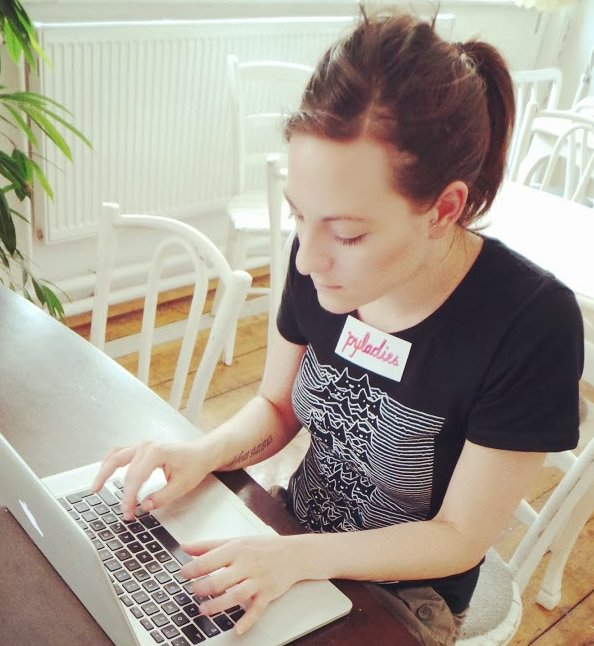
\includegraphics[width=\linewidth]{laura/laura-sitting.jpg}
\footnotesize{Laura Gaetano. Bildrechte: [1]}
\end{center}

\textbf{Laura Gaetano}, im Internet bekannt als \href{http://www.alicetragedy.org/blog/}{\textit{AliceTragedy [1]}} arbeitet in Wien als Junior Developer und Social Media Expertin bei \href{http://bitstem.com}{\textit{Bitstem [2]}}. Seit Ende 2013 organisiert sie die Pyladies Vienna Meetings. Folgendes \href{http://www.alicetragedy.org/blog/?p=6271}{\textit{Blogposting [3]}} schrieb sie im Oktober 2013. Übersetzung von \href{http://spielend-programmieren.at}{\textit{Horst JENS [4]}}. \\

(Beginn der Übersetzung) \\

\subsection*{Es war einmal, in einer weit, weit entfernten Galaxie...}

Ich habe das Schreiben dieses Blog-Postings lange vor mir her geschoben. Das Leben ist ein so viel netterer Platz als das Internet in letzter Zeit, also habe ich lieber das Leben genossen als es still vom Rande aus zu beschreiben wie ich das sonst mache.

Für die (paar) die es interessiert, hier ist eine kleine Zusammenfassung der letzten Monate:

\subsection*{RailsGirls:}

Ich besuchte den RailsGirls Event im Jänner, und er hat mein Leben verändert. Ich sah dort eine Menge Dinge die Frau verbessern könnte um das Erlebnis als Besucherin angenehmer zu machen. Deshalb besuchte ich im August zum ersten Mal überhaupt einen \textbf{RailsGirls} Event \href{http://railsgirls.com/bratislava}{\textit{als Trainerin, in Bratislava [5]}}. Dieses Wochenende war ich auch seit sechs Monaten in meinem neuen Job. Wirklich ? Ein halbes Jahr kämpfe ich mich schon täglich mit \textbf{Ruby on Rails} ab? Wer hätte vor neun Monaten gedacht dass ich einmal von Stadt zu Stadt reisen würde um Vorträge über die \textbf{Kommandozeile} zu halten ? 

Aber es gibt für Alles ein erstes Mal und ich lernte einige wirklich großartige und interessante Leute kennen, ich lernte besser in der Öffentlichkeit Vorträge zu halten, und ich bekam gratis Aufkleber. Vor allem: Ich freue mich immer so zu sehen wenn wenigstens eine meiner 'Schülerinnen' sich für das Programmieren begeistert (get excited about making stuff) und sich ernsthaft überlegt in dieser Richtung zu arbeiten.   

\begin{center}
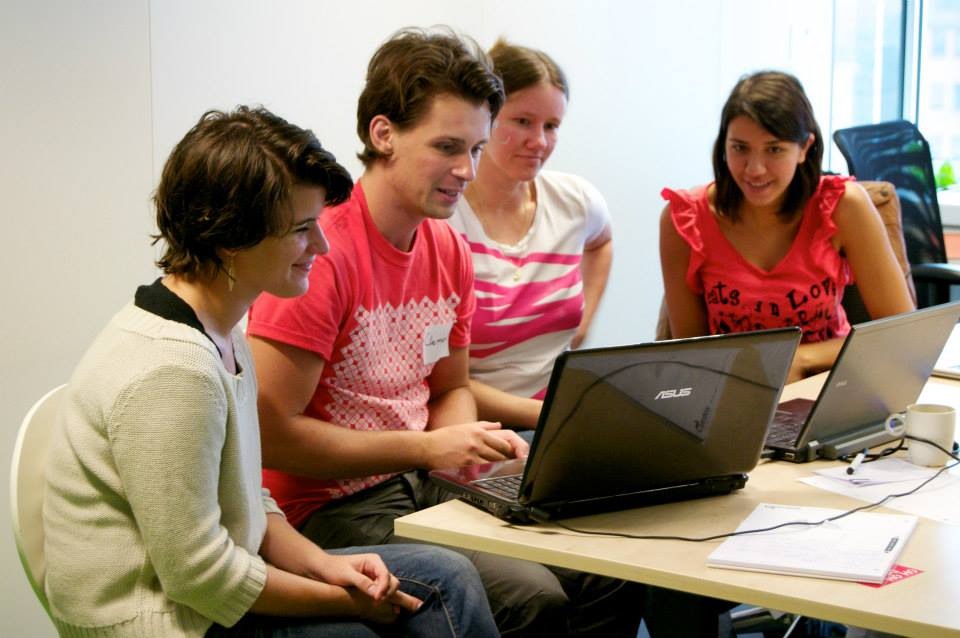
\includegraphics[width=\linewidth]{laura/floor_rg_thehague_3.jpg}
\footnotesize{Rails-Treffen The Hague. Bildrechte: [1]}
\end{center}


(Nebenbemerkung: In letzter Zeit gab es einiges Aufsehen über das Thema \textbf{Sexismus} in der Technologie-Branche. Ich denke man kann nicht genug darauf hinweisen dass dies nichts speziell mit der Ruby Community zu tun hat, oder mit Programmieren im Allgemeinen, oder mit der \textbf{IT-Industrie}. Sexismus, und jede andere Form von Diskriminierung, ist unglücklicherweise ein weltweites, branchenübergreifendes Problem. Es ist traurig, aber ich denke es hilft nicht das wir Frauen uns als Opfer betrachten. Vielleicht ist der Effekt von Organisationen wie RailsGirls die Frau welche Teil der IT-Industrie werden will öffentlich zu machen und das Problem damit größer zu machen als es eigentlich ist; Ich weiß es nicht. Für mich war \textbf{RailsGirls} der erste Schritt in Richtung Programmieren und ich möchte diese positive Erfahrung an andere zurück geben.)

\subsection*{Meetups:}

Momentan ich ich regelmäßige Besucherin der \href{http://vienna.rb}{\textit{Vienna.rb [6]}} Meetups und der \href{http://wpvienna.com/}{\textit{WordPress Vienna [7]}} Meetups in Wien. Die Meetups fühlen sich fast so nett an wie ein Familientreffen, deshalb schlage ich vor ihr besucht uns wenn ihr Interesse daran habt mit netten Leuten zusammen zu sein und Programmieren zu lernen. \href{http://meetup.com/pyladies-vienna}{\textit{Pyladies Vienna [8]}}, welches ich zusammen mit \textbf{Floor DREES}\footnote{Siehe Artikel \texttt{floor} in dieser Ausgabe} organisiere, findet auch bald statt. 

\subsection*{750 Wörter:}

Vor Jahren, ich ging noch ins Gymnasium, fand ich ein Buch über 'kreativ Schreiben' welches empfahl täglich zu schreiben. Nicht notwendigerweise gut konstruierte kleine Essays oder Geschichten; aber trotzdem drei volle Seiten täglich (die 'morning pages') ohne zu viel über den Inhalt nachzudenken. Der Grund dafür ist dass dies dabei hilft die \href{https://de.wikipedia.org/wiki/Schreibblockade}{\textit{Schreibblockade}} zu mindern. 

Einige Jahre später nahm ich an \href{http://nanowrimo.org/}{\textit{Nanowrimo} [9]} teil und bald darauf meldete ich mich bei \href{https://750words.com/}{\textit{750 Words}} an, inspiriert durch meine Schreibübungen. 750 Words erlaubt dem user täglich Seiten zu schreiben, führt Statistiken über Schreibgeschwindigkeiten und Stimmungen, und man kann Abzeichen (badges) gewinnen. 

Als ich in Bratislava war beschloss ich am monatlichen 750words Wettbewerb teilzunehmen: Ich habe seitdem nicht mehr aufgehört zu schreiben und finde jeden Tag 15 bis 20 Minuten Zeit dafür. Ironischerweise blogge ich seitdem deutlich weniger, aber man kann nicht alles gleichzeitig machen. 

\subsection*{Und jetzt ?}

Ich lese einen Haufen Sachbücher (Gay Talese und Norman Mailer sind gerade meine Favoriten), ich verbessere meine \textbf{Typografie} Kenntnisse und versuche langsam \textbf{Javascript} in meinen Kopf hinein zu bekommen weil ich Javascript noch überhaupt nicht kann. Außerdem verfolge ich ein paar Nebenprojekte. Und ich habe erstmals in meinem Leben \textbf{GTA} gespielt (ich weiß, unakzeptabel, aber wozu gibt es einen Freund mit Playstation?). Und obwohl ich nur sporadisch blogge bleibt Blogs schreiben meine erste Liebe zu der ich hoffentlich bald zurück komme. 

(Ende der Übersetzung)

\subsection*{Anmerkungen}
\textbf{Alterslimit:} \\
Laut Laura gibt es weder für Rails Girls noch für Pyladies Treffen ein Alterslimit, die ältesten Teilnehmerinnen bisher waren über 50. Mit minderjährigen  Teilnehmerinnen hat sie noch keine Erfahrung und ersucht bei der Anmeldung extra auf das Alter hinzuweisen, um die Organisation zu erleichtern.

\textbf{Vorträge:} \\
Wer auf einem (Pyladies) Treffen einen sogenannten Lightning-Talk halten will (max. 5 Minuten, sehr empfehlenswert) möge Laura im Vorfeld kontaktieren. 


\subsection*{Fachbegriffe}

\textbf{RailsGirls} Internationaler Verein, organisiert Treffen für Frauen welche die Programmiersprache \textbf{Ruby on Rails} lernen möchten. \\

\href{https://en.wikipedia.org/wiki/Ruby_on_rails}{\textbf{Ruby on Rails}} ist ein \textit{open source web application framework}, geschrieben in der Programmiersprache \href{ruby}{\textbf{Ruby}}. 

\href{https://en.wikipedia.org/wiki/Ruby_(programming_language)}{\textbf{Ruby}} ist eine \textit{general-purpose programming language} ähnlich wie \textbf{Python} \\

\textbf{Kommandozeile, command line} Text-Eingabemethode im Unterschied zu grafischen User Interfaces (GUI), welche mit der Maus bedient werden. Die Kommandozeile wird vor allem von Programmierern bevorzugt da man damit im Unterschied zu einem GUI deutlich schneller arbeiten kann (wenn man sich auskennt). \\

\href{https://de.wikipedia.org/wiki/Sexismus}{\textbf{Sexismus}} Diskriminierung aufgrund des Geschlechts. In der IT-Branche ist damit meist die Diskriminierung von Frauen gemeint. \\

\textbf{IT-Industrie} Internet-Technologie \\

\href{https://twitter.com/pyladies_vie}{\textbf{Pyladies Vienna} [8]} steht für Python Ladies, eine Selbstlerngruppe für die Programmiersprache  \textbf{Python} speziell für Frauen. \\

\href{http://python.org}{\textbf{Python}} leicht zu erlernende general purpose Programmiersprache \\

\textbf{Wordpress} populäre Opens-Source Software um Webseiten, speziell \textbf{Blogs}, zu erstellen \\

\textbf{Blog} eine öffentlich sichtbares 'Tagebuch' (Logbuch) im Internet. \\

\textbf{Typografie} Druckkunst, gestalterische Merkmale eines Schriftsatzes. \\

\textbf{Javascript} Programmiersprache (nicht zu verwechseln mit Java) die innerhalb eines Browserfensters läuft. \\

\textbf{Grand Theft Auto}, GTA: Sehr populäre Computerspiel-Serie 

\subsection*{Download, Feedback:}
\footnotesize{
Download: Ordner \texttt{laura} \Mundus\ \href{http://spielend-programmieren.at/risjournal/001}{spielend-programmieren.at/risjournal/001}\\
Startseite:\\
\href{http://spielend-programmieren.at/de:ris:001:start}{spielend-programmieren.at/de:ris:001:start}\\ 
\Letter\:  girl@alicetragedy.org \\}
\normalsize
 

\subsection*{Lizenz, Quellen:}

\begin{wrapfigure}{l}{2.0cm}

\includegraphics[width=2cm]{ccbysa88x31.png}
\end{wrapfigure}
Dieses Material steht unter der Creative-Commons-Lizenz Namensnennung - Weitergabe unter gleichen Bedingungen 4.0 International. Um eine Kopie dieser Lizenz zu sehen, besuchen Sie \url{http://creativecommons.org/licenses/by-sa/4.0/deed.de}.

\textbf{Quellen}: \\
{[}1{]} \href{http://www.alicetragedy.org/blog/}{www.alicetragedy.org/blog/} \\
{[}2{]} \href{http://bitstem.com}{bitstem.com} \\
{[}3{]} \href{http://www.alicetragedy.org/blog/?p=6271}{goo.gl/WG7AvI} \\
{[}4{]} \href{http://spielend-programmieren.at}{spielend-programmieren.at} \\
{[}5{]} \href{http://railsgirls.com/bratislava}{railsgirls.com/bratislava} \\
{[}6{]} \href{http://vienna-rb.at/}{vienna.rb} \\
{[}7{]} \href{http://wpvienna.com/}{wpvienna.com} \\
{[}8{]} \href{http://www.meetup.com/pyladies-vienna}{meetup.com/pyladies-vienna} \\
{[}9{]} \href{http://nanowrimo.org/}{nanowrimo.org/} \\
{[}10{]} \href{https://750words.com/}{750words.com/} 


\end{multicols}
\SepRule
%-----------------------------------------------------------
\end{document}